%-------------------------------------------------------------------------------
\section{Problem}\label{s:problem}
%-------------------------------------------------------------------------------


The problem is that \cgroups{} does not provide an interface that is conducive
to the goals that Kubernetes has. 

In Kubernetes, both CPU requests and limits are expressed as an amount of
milliCPU. For CPU requests, each pod should have access that amount of CPU,
which is reserved for that pod whenever it is placed on a node. This number may
be 0, in which case the pod is BestEffort and may get no CPU time. For CPU
limits, the pod should be throttled if it tries to use more than the amount of
CPUs it is limited to.

The interface Kubernetes uses to enforce these promises is \cgroups{}, of which
it uses two features: weight and max. We show that the promises weight and max
make do not add up to the promises Kubernetes makes, and why they are not
conducive to the paradigm of enforcing a guaranteed minimum reservation with
potential bursting that Kubernetes as well as others expose to end users.


\subsection{\cgroups{}' cpu.weight fails to enforce Kubernetes' idea of requests}

Kubernetes uses the \cgroups{} weight interface to enforce pods' CPU requests.
It makes sure that machines are never oversubscribed on requested CPU, and then
uses weights to split up the cores on the machine.

Kubernetes put BestEffort pods into a group with the lowest possible weight,
which is 1. Burstable and Guaranteed pods are given a weight that is calculated
based on the number of cores the machine has and how many CPUs the pod
requested. For instance, on a 56 core machine we found that a pod that requested
4 cores was given a weight of 157, whereas one that request 2 CPUs was given a
weight of XX.

However, we find that the weight interface fails to enforce these pods' requests
because of one key observation: \textit{weights are a local property}. Linux
maintains a separate runqueue on each core, in order to avoid the overheads of
accessing global state for every scheduling decision. Within each runqueue,
Linux's scheduler works to maintain the correct ratio of received CPU time at
each scheduling; but Linux does not enforce the weight ratios across cores. This
leads to two important problems. 


\subsubsection{BestEffort pods run more than they should}

\begin{figure}[t]
    \centering
    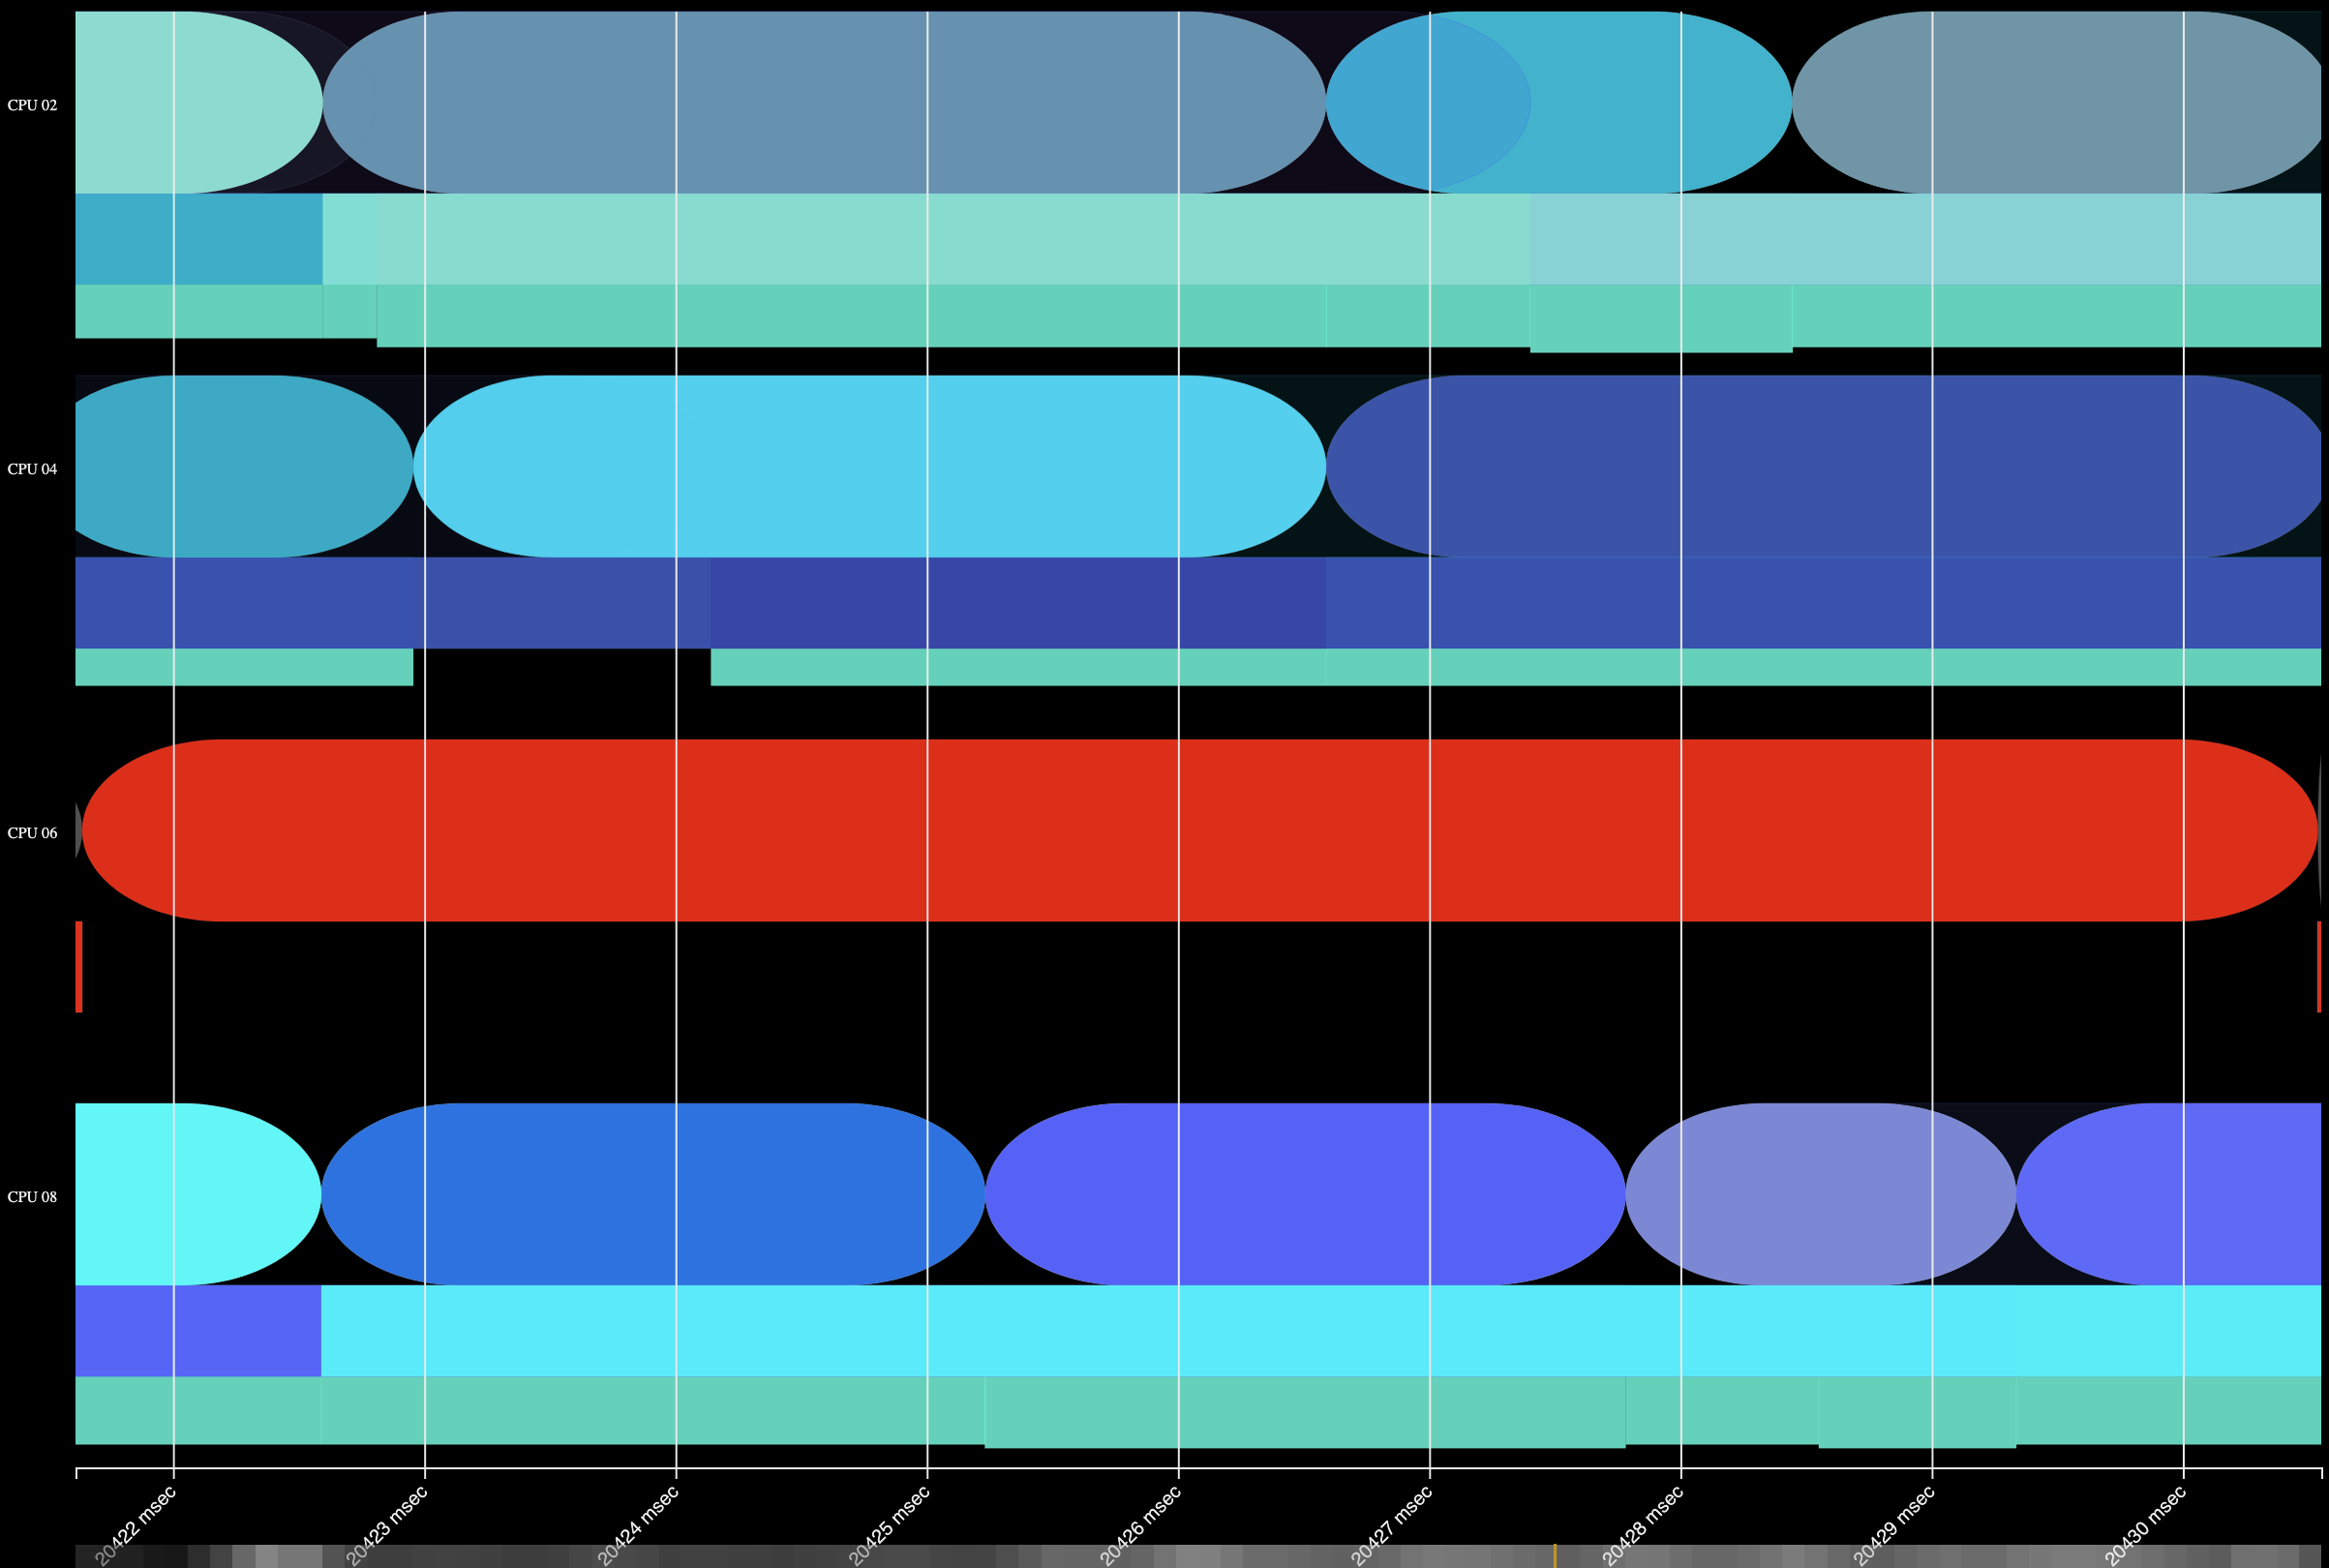
\includegraphics[width=\columnwidth]{graphs/schedviz-be-problem.png}
    \caption{Core 6 runs an image resize process, unaware that cores 2, 4, and 8
    all have runnable and queued server threads}\label{fig:schedviz-be-problem}
\end{figure}

One problem is with using a very small weight to run BestEffort pods. Because
the weight is only enforced per-core, this can lead to a situation where that
\textit{one core is running a best effort process, while threads of processes
with resource reservations are queued on another}. This is because the threading
model of the server interacts with the per-core runqueues. The server uses a
pool of worker threads (one per client). The number of threads that the server
has is larger than the number of cores, which means that each core has multiple
server threads. It occasionally occurs that all the current requests are on
server threads that happen to be on only three of the four available cores,
which leaves one runqeueue with only idle server worker threads. This leads to
an inversion, where the core that has no runnable high weight server threads and
thus runs a low weight one, while other cores have queued high weight processes.

\autoref{fig:schedviz-be-problem} shows this occuring in a trace from the
experiment running an image resize job along the web server, from which we
visualize the perf trace using schedviz~\cite{schedviz-tool}. The process
running on each core is shown as an oval, and queued processes are shown as
rectangles below; the x-axis is time and the y-axis shows the 4 cores the
experiment is running on. We see that on core 6, the red process that is running
for the whole 10ms is a thread of the image resize job, while server threads,
shown in varying shades of blue, are queued on the other cores. 

Load balancing eventually remedies the inversion by migrating runnable
high-weight threads to the under-loaded core. However, load balancing runs
significiantly less frequently than scheduling does, at least during high load.
How often load balancing runs in general is a complicated number that is
dependent on how close the two cores are in the CPU architecture hierarchy, as
well as how loaded the machine is.

\begin{figure}[t]
    \centering
    \begin{subfigure}{\columnwidth}
        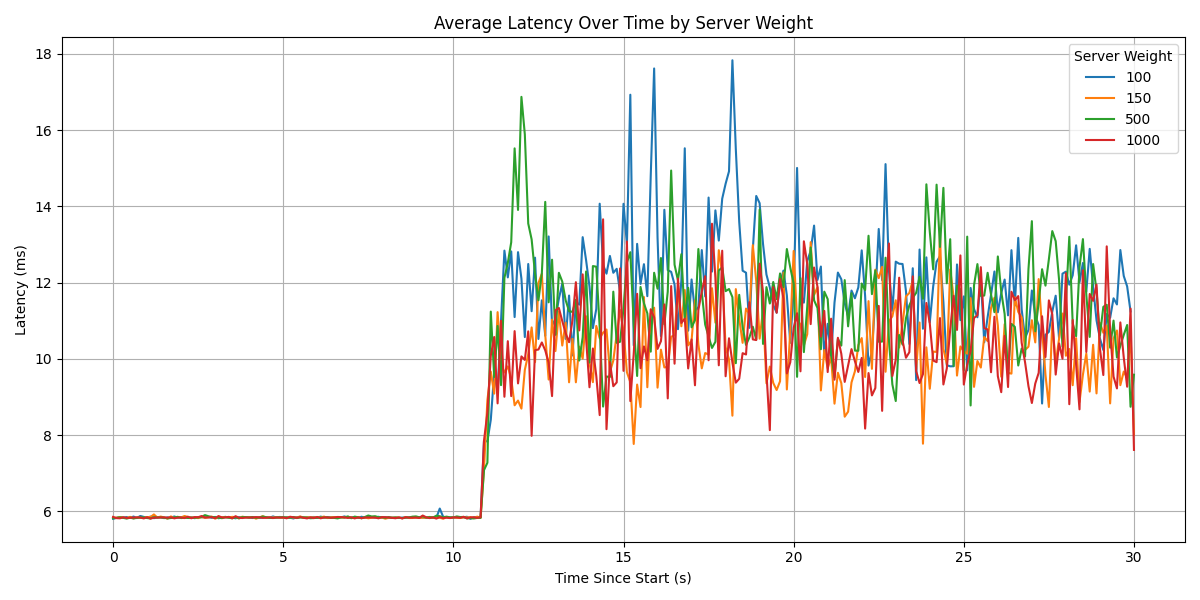
\includegraphics[width=\columnwidth]{graphs/srv-bg-weight-cmp-low.png}
        \caption{Low load stetting, utilization before starting the BE tasks is
        around 85\%}\label{fig:srv-bg-weight-cmp-low}
        \vspace{12pt}
    \end{subfigure}
    \hspace{\fill}
    \begin{subfigure}{\columnwidth}
        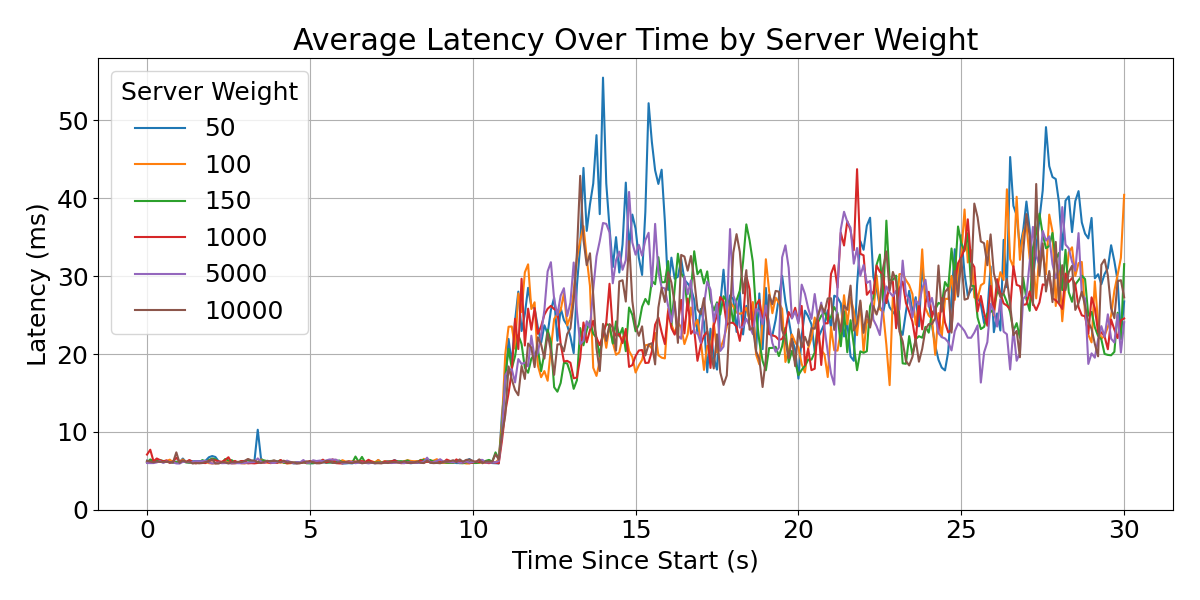
\includegraphics[width=\columnwidth]{graphs/srv-bg-weight-cmp-high.png}
        \caption{High load setting, utilization before starting the BE tasks is
        around 95\%}\label{fig:srv-bg-weight-cmp-high}
    \end{subfigure}
    \vspace{4pt}
    \caption{Changing the weight of the server beyond 100 has little impact on
    how much the weight 1 best effort task interferes with it}\label{fig:srv-bg-weight-cmp}
\end{figure}

This inversion has a large effect, to the point of making weight ratios above a
certain range ineffective across cores. We demonstrate this with a
microbenchmark, which runs a simple CPU-bound server with a pool of worker
threads. We run an open-loop client on a remote machine, and then start two best
effort workloads doing image resizing. We put the server and the image resize
job each in their own \cgroups{} group, and pin them to the same set of four
cores. The image resize job always has weight 1, and we vary the weight of the
server. \autoref{fig:srv-bg-weight-cmp} shows that using a bigger weight split
has no impact on the latency impact of the best effort task. For all the
weights, at a $\sim$85\% baseline utilization of the server the server's mean
latencies spike up from steady at around 6ms to $\sim$15ms, and much higher for
99th percentile latencies. At a baseline utilization of 95\%, those numbers
increase to up to 40ms for the the mean latency, and 80ms for the tail.


\subsubsection{Burstable and Guaranteed pods share each core by weight}

The other problem is that pods with requests, ie Burstable and Guarnateed pods,
share cores where they both have threads based on weight, irrespective of who is
running how much on other cores.


\begin{figure}[t]
    \centering
    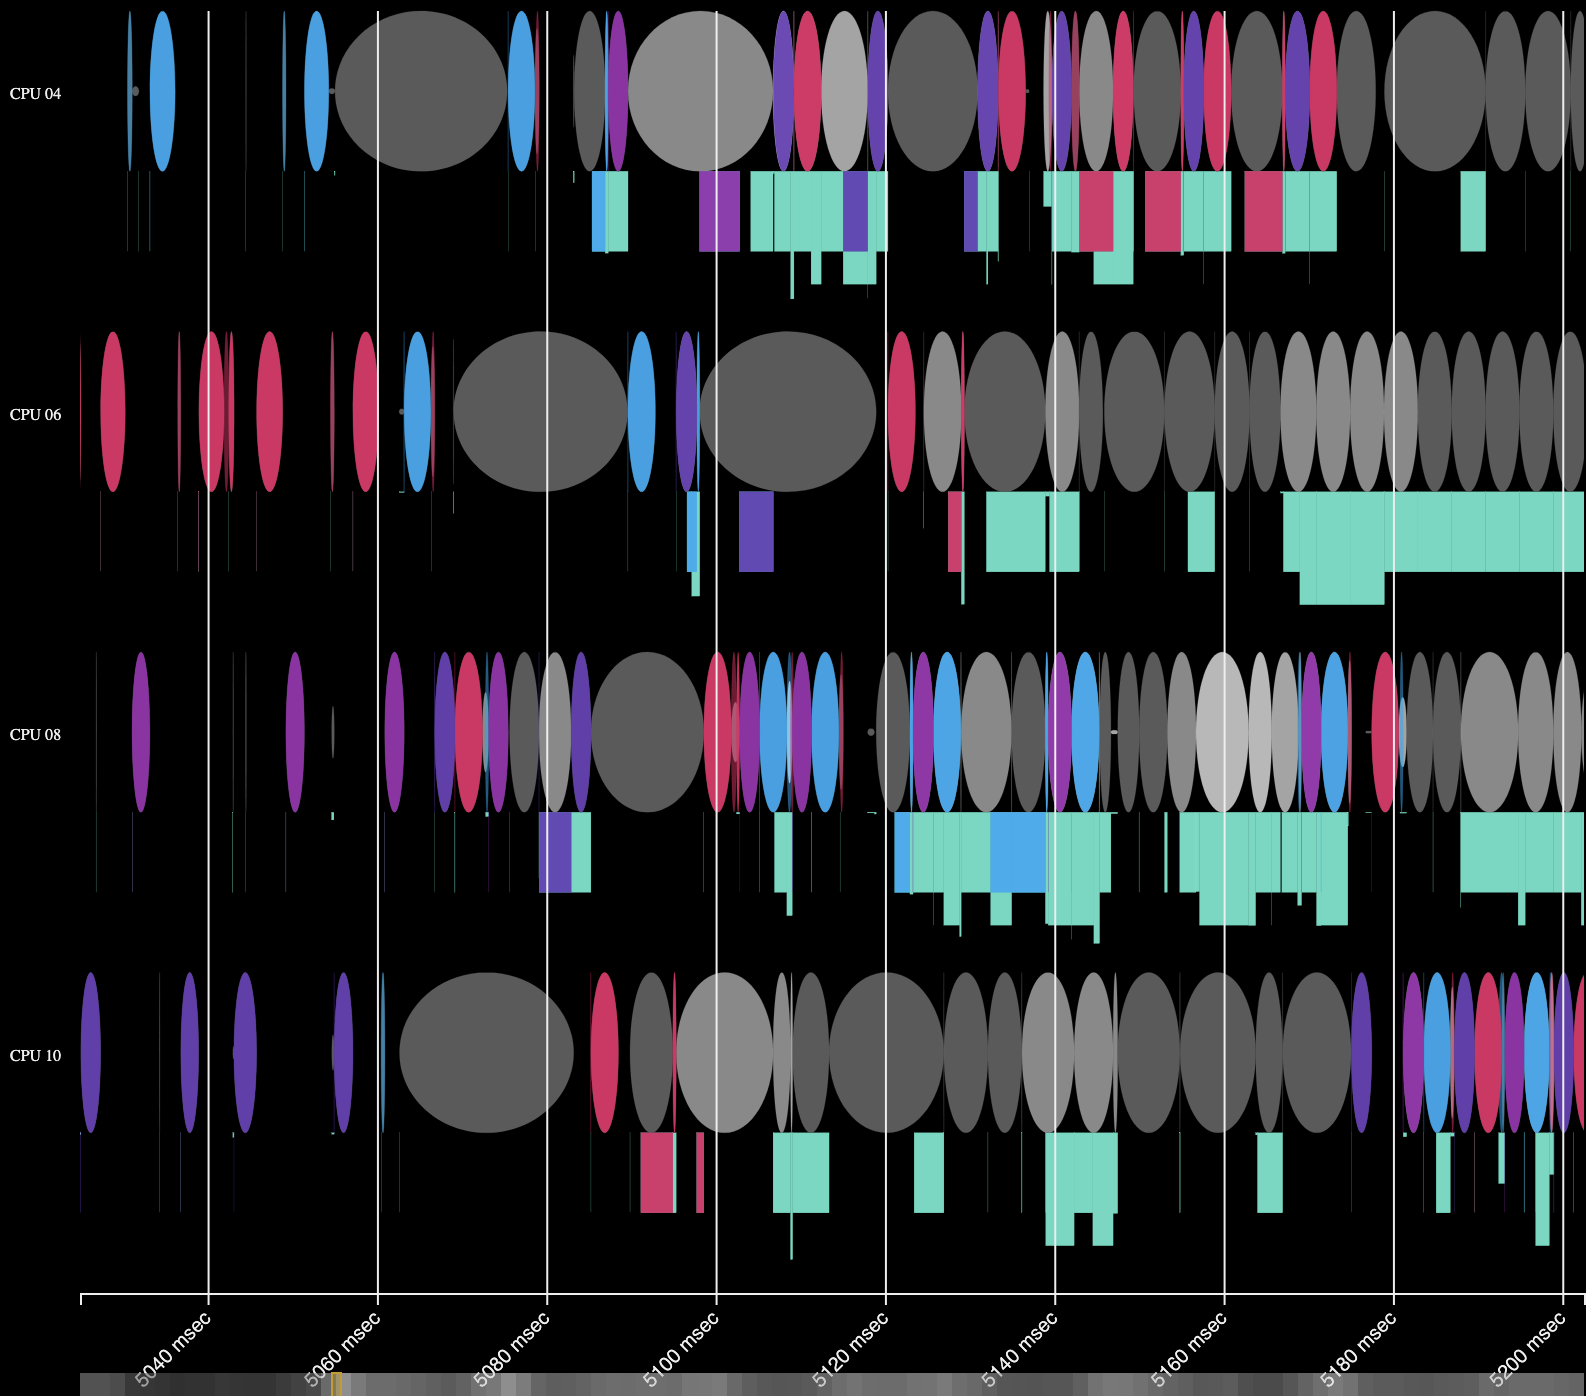
\includegraphics[width=\columnwidth]{graphs/schedviz-lc-burst-problem.png}
    \caption{When server1 is running alone, it has all the cores to itself, but
    after server2 starts it gets only half of whatever core it runs on, even if
    that is a fraction of the cores available and server2 is running uncontended
    on the other cores}\label{fig:schedviz-lc-burst-problem}
\end{figure}

Suppose, as in the experiment from \autoref{fig:kubernetes-lc-burst}, two
servers have the same amount of requested CPU, but different amounts of load.
The server with less load will have less runnable threads. However, on the few
cores where its threads are runnable, it will have to share that core equally;
even while the server with higher load runs uncontended on other cores.
\autoref{fig:schedviz-lc-burst-problem} shows this happening: on the left hand
side of the trace, server1 can run uncontended on any core when requests come
in. Then server2 starts, and has a high load and thus immediately starts running
on all four cores, because it is Burstable. When a request from server1 comes
in, the thread processing that request has to share the core equally with
threads from server2, even while server2 gets other cores all to itself.



\subsection{\cgroups{} cpu.max fails to enforce Kubernetes' idea of limits}


The interface to \cgroups{} cpu.max is already different from that of
Kuberentes' milliCPUs: \cgroups{} asks instead for a runtime $r$ and a period
$p$, and ensures that the group never gets more than $r$ CPU time per $p$ time
period. Because multi-threading is a thing, it is possible that $r>p$. 

\begin{figure}[t]
    \centering
    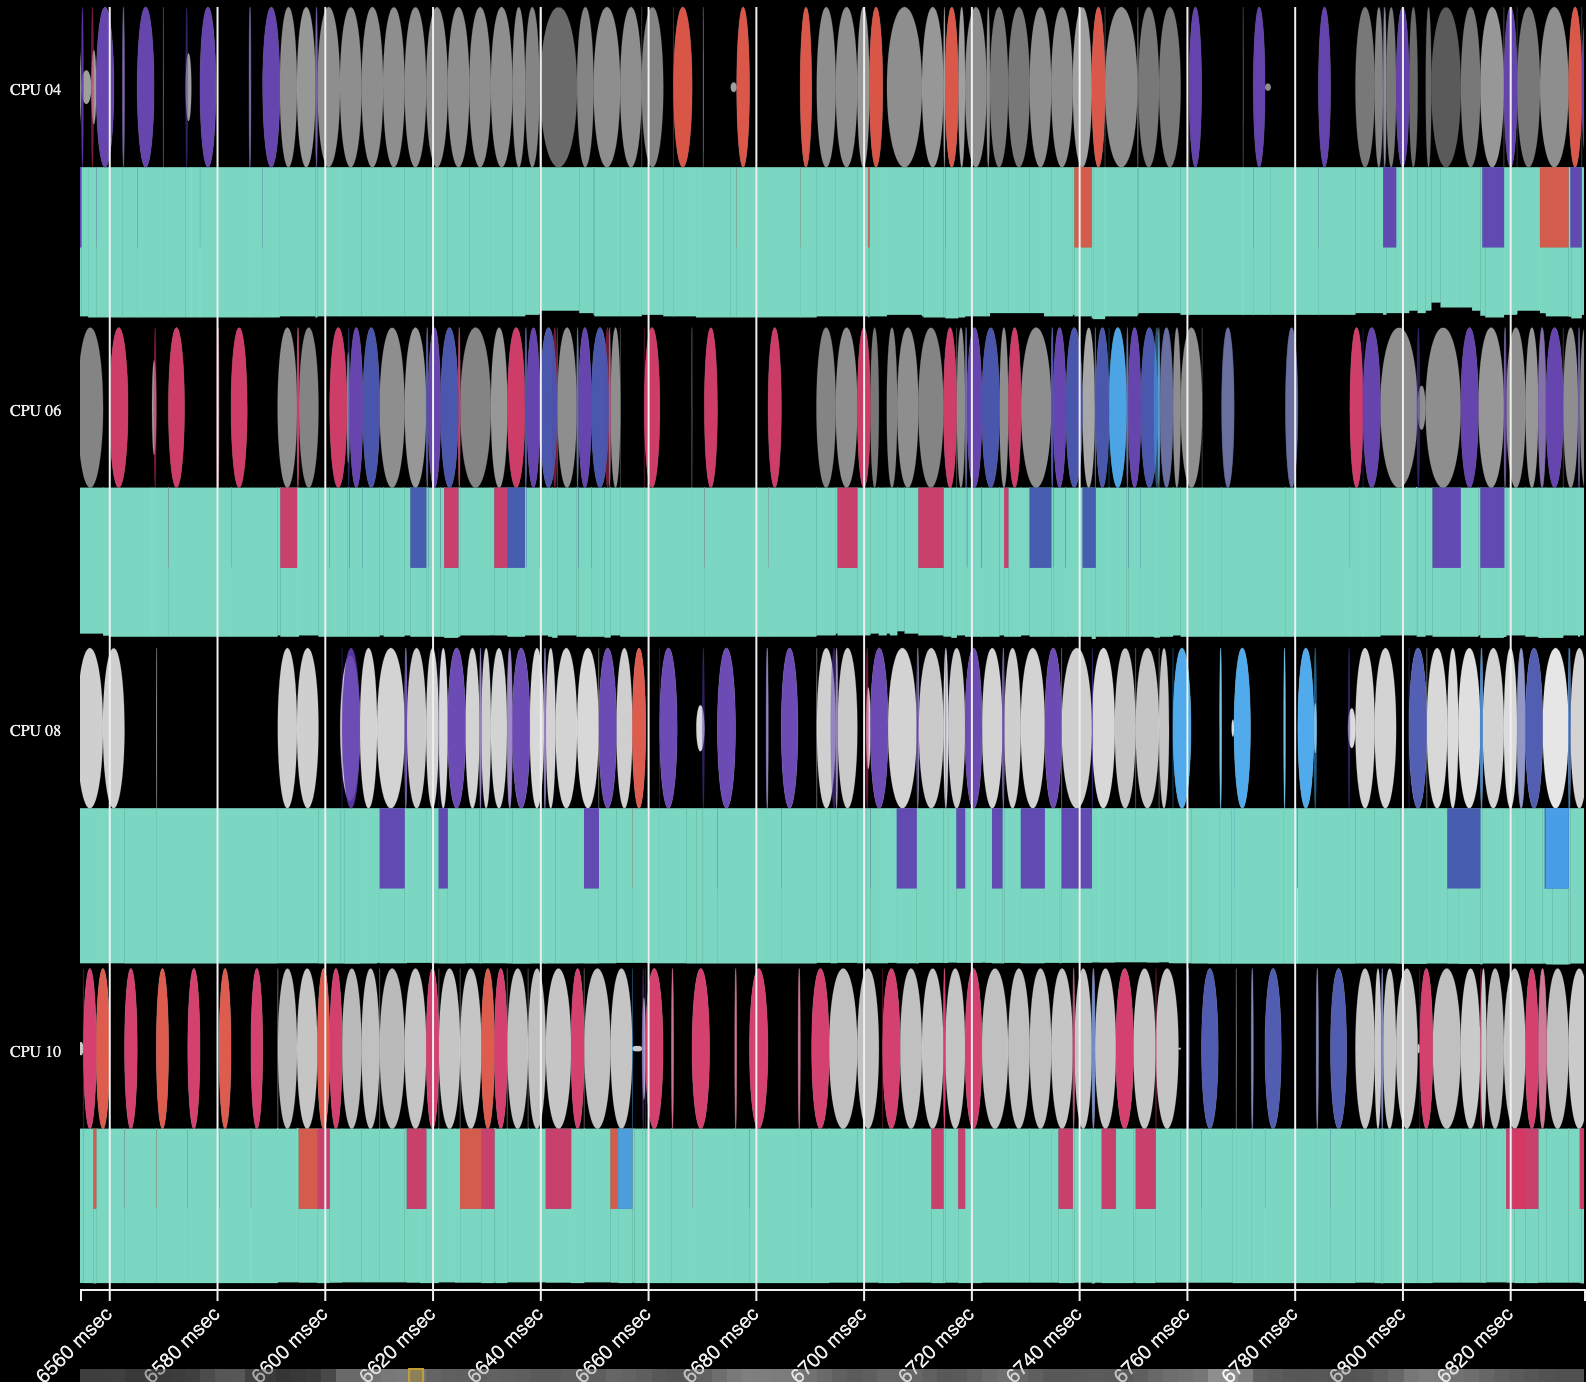
\includegraphics[width=\columnwidth]{graphs/schedviz-lc-guar-problem.png}
    \caption{When server1 is running alone, it has all the cores to itself, but
    after server2 starts it gets only half of whatever core it runs on, even if
    that is a fraction of the cores available and server2 is running uncontended
    on the other cores}\label{fig:schedviz-lc-guar-problem}
\end{figure}

However, enforcing a limit of 2 vCPUs is different than enforcing that a group
only get 2ms of CPU time every ms. If a pod is restricted to 2vCPUs, then it can
run up to two things at the same time, and thus use only up to two cores.
However, if a group is limited to 2ms every ms, it could also fill its quota by
running four things on four cores for half a ms. In the time when one group is
running on all four cores, Kubernetes relies on weights to separate the two,
which can lead to significant delays for other services, as we saw.
\autoref{fig:schedviz-lc-guar-problem} shows this happening in a trace from the
experiment from \autoref{fig:kubernetes-lc-guar}. We can see the phases of
servive2 threads in grey, which run for a while on all four cores, disrupting
the blue server1 threads, before being throttled, during which time server1
threads can run uninterrupted and otherwise the cores lie idle.



% \subsection{Enforcing weights across cores is
% hard}\label{ss:problem:cross-core-hard}

% A weight-based interface is at odds with machine-wide policy enforcement. In
% order to globally enforce a processes weight, the scheduler would need to
% look at every cores' runqueues at every scheduling decision. 

% This check needs to happens at every tick because, in a weight-based system, the
% definition of what process should be running changes over time. If a core has
% one high-weight and one low-weight group, before running the low-weight group it
% needs to know if any other cores have recently run a different process within
% that group, because that would affect how much time it is owed on this core.

% Enforcing weights across cores is expensive: looking at remote queues at each
% scheduling decision removes the benefit of having local runqueues. Inter-core
% communication and having every core look at every other cores' runqueues can
% lead to contention, which has been demonstrated to be a bottleneck for
% performance at scale~\cite{afaas}. This means that the overheads of maintaining
% a weight split as a global invariant can quickly become prohibitive.

% On top of the communication cost, managing and calculating global shares is
% complex: calculating whether a given process is owed time globally requires
% knowing the total weight across all cores as well as the sum of time that all
% the processes in the group have gotten. Such a calculation would include
% complicated accounting that takes into account, amount other things, different
% cores' virtual times, processes' weights, groups, and limits. Just within
% runqueues the accounting is already so complicated that comments in the Linux
% source include function derivations and equation rewriting.


% \subsection{Weights interact poorly with tick-based
% scheduling}\label{ss:problem:quantum}

% Even on a single runqueue, in a weight based scheme best effort processes need
% to get a fair share of the CPU. The problem is that, when this happens, the BE
% process will interrupt any running LC process for a whole tick. In Linux,
% hardware ticks are 4ms long. This means that a thread that has a CPU reservation
% and is processing a request may be interrupted for up to 4ms by a best effort
% process, provided the latter runs that long before blocking. 4ms can be a large
% amount of time for microservice workloads, whose SLOs are often in the low
% double digit or even single digit ms realm.~\cite{in-the-plex, sigmaos}



